\documentclass[letterpaper, 28pt, fleqn]{article}
%%%%%%% PACKAGES %%%%%%%%
\usepackage[utf8]{inputenc}
\usepackage[margin=1.5cm]{geometry}
\usepackage{blindtext}
\usepackage{setspace}
\usepackage{multicol}
\usepackage{graphicx}
\usepackage{palatino}
\usepackage{booktabs}
\usepackage{listings}
\usepackage{url}
\usepackage{hyperref}
\usepackage{notoccite} %citation number ordering
\usepackage{lscape} %landscape table
\usepackage{caption} %add a newline in the table caption
\usepackage[breakable]{tcolorbox}
\usepackage[toc,page]{appendix}
\usepackage{graphicx}
\graphicspath{ {./images/} }
\usepackage{fancyvrb} % verbatim replacement that allows latex
\usepackage[
backend=biber,  %references format (IEEE)
style=ieee,
sorting=none
]{biblatex}
\usepackage{color}

\definecolor{dkgreen}{rgb}{0,0.6,0}
\definecolor{gray}{rgb}{0.5,0.5,0.5}
\definecolor{mauve}{rgb}{0.58,0,0.82}

\definecolor{codegreen}{rgb}{0,0.6,0}
\definecolor{codegray}{rgb}{0.5,0.5,0.5}
\definecolor{codepurple}{rgb}{0.58,0,0.82}
\definecolor{backcolour}{rgb}{0.95,0.95,0.92}

\addbibresource{refs.bib} %rename this to your own bibliography


    \definecolor{incolor}{HTML}{303F9F}
    \definecolor{outcolor}{HTML}{D84315}
    \definecolor{cellborder}{HTML}{CFCFCF}
    \definecolor{cellbackground}{HTML}{F7F7F7}
        % prompt
    \makeatletter
    \newcommand{\boxspacing}{\kern\kvtcb@left@rule\kern\kvtcb@boxsep}
    \makeatother
    \newcommand{\prompt}[4]{
        {\ttfamily\llap{{\color{#2}[#3]:\hspace{3pt}#4}}\vspace{-\baselineskip}}
    }
    
    
% Pygments definitions
\makeatletter
\def\PY@reset{\let\PY@it=\relax \let\PY@bf=\relax%
    \let\PY@ul=\relax \let\PY@tc=\relax%
    \let\PY@bc=\relax \let\PY@ff=\relax}
\def\PY@tok#1{\csname PY@tok@#1\endcsname}
\def\PY@toks#1+{\ifx\relax#1\empty\else%
    \PY@tok{#1}\expandafter\PY@toks\fi}
\def\PY@do#1{\PY@bc{\PY@tc{\PY@ul{%
    \PY@it{\PY@bf{\PY@ff{#1}}}}}}}
\def\PY#1#2{\PY@reset\PY@toks#1+\relax+\PY@do{#2}}


\lstset{frame=tb,
  language=python,
  backgroundcolor=\color{backcolour},  
  commentstyle=\color{codegreen},
  keywordstyle=\color{magenta},
  numberstyle=\tiny\color{codegray},
  stringstyle=\color{codepurple},
  basicstyle=\ttfamily\normalsize,
  breakatwhitespace=false,         
  breaklines=true,                 
  keepspaces=true,                 
  numbers=left,       
  numbersep=5pt,                  
  showspaces=false,                
  showstringspaces=false,
  showtabs=false,                  
  tabsize=2,
  framesep=20pt,
  xleftmargin=10pt,xrightmargin=10pt,
  columns=fullflexible,
  frame=none
}

\author{Yadhu Krishna M \\
\texttt{yadhukrishna.mpm@gmail.com}
}

\begin{document}
\pagenumbering{roman} % Start roman numbering

\title{Machine Learning - 19CSE305 \\ \huge{\textbf{Phishing URL Detection using Machine Learning}}}

\setlength{\columnsep}{0.45in}

\setcounter{page}{1}

\pagenumbering{arabic} % Start roman numbering

\maketitle

%%% CONTENT HERE %%%%
\begin{multicols}{2}
\section{Problem Definition}

The project aims to build a machine learning model that would predict whether a given Uniform Resource Locator (URL) is a potential phishing link (Task). The algorithm would be trained using a dataset of URLs in which some are phishing URLs and others are legitimate ones (Experience). 


\section{Dataset Used}

The dataset used in this project contains 11430 URLs out of which 50\% are phishing and 50\% legitimate URLs. It has 87 extracted features out of which 56 are extracted from the structure and syntax of URLs, 24 extracted from the content of their correspondent pages, and 7 extracted by querying external services. \\
The following are some of the major features present in the dataset. 
\begin{enumerate}
\item Length of URL 
\item Length of hostname
\item Use of any URL shortening service
\item Suspicious TLD
\item No of redirections - external or internal
\item Number occurrences of special characters in URL
\item Search Index ranking
\end{enumerate}

Three other datasets were also used for the same project, and would be documented in other submissions.

\section{Data Pre-processing}

This section describes the steps that were done to pre-process the data. 


\begin{itemize}
    \item Most of the features in the dataset contained numerical values indicating features that were derived from a URL string. 
\item The result column initially contained non-numeric values which were used to indicate legitimate and phishing URLs. This column was mapped into 0 and 1 respectively. 
\item Since this project was focused on only features derived from URL such as length of URL, number of special characters etc. So, other features in the dataset such as results from third-party services (results from search engine, WHOIS lookups etc.) were omitted.
\item The dataset was checked for null values, and duplicate entries however, no such records were observed.
\item Normalization was performed using MinMax scaler on the entire dataset. 
\end{itemize}



\section{Data Summarization}

This section describes the use of statistical methods applied to breakdown, and understand the data.

The dataset was inspected and it was observed to contain 11,430 unique entries after preprocessing. The number of features were reduced to 34. There were 33 features extracted from the URL, and a column indicating whether the entry was that of a legitimate or a phishing URL. 
On grouping the dataset by the result, it was identified that the dataset was properly balanced, and it contained 50\% legitimate and 50\% phishing URLs. There were 5,715 legitimate and phishing URLs. 

Code used for summarizing this data has been uploaded to the project folder.

\begin{figure*}
  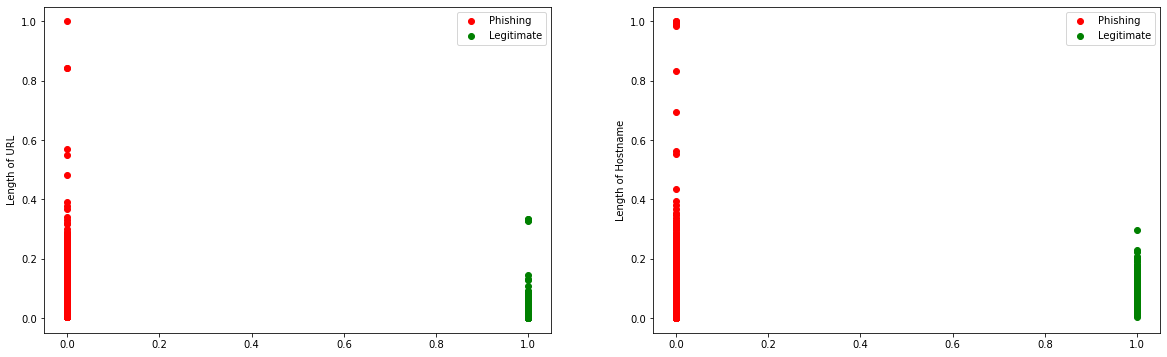
\includegraphics[width=\linewidth]{scatter_plot_1}
  \captionof{figure}{Scatter Plot depecting how length of URL varies in legitimate and phishing URLs.}
  \label{fig:scatter1}
\end{figure*}


\section{Data Visualization}

After summarizing the data, two types of graphs - a scatter plot and a double bar graph were plotted to better understand how each feature affected the result.  \\

The dataset was divided into two classes - \textbf{legitimate} and \textbf{phishing} to easily inspect the data.
One of the main features of the dataset was the length of URL and the length of hostname. Phishing websites are normally said to have long URLs to hide certain parts of the URL. A scatter plot was drawn to see the  visibility of this feature  in the dataset. \\

Double bar graphs were also plotted to compare how the remaining features varied for both the classes. 


\begin{Figure}
	
 \centering
 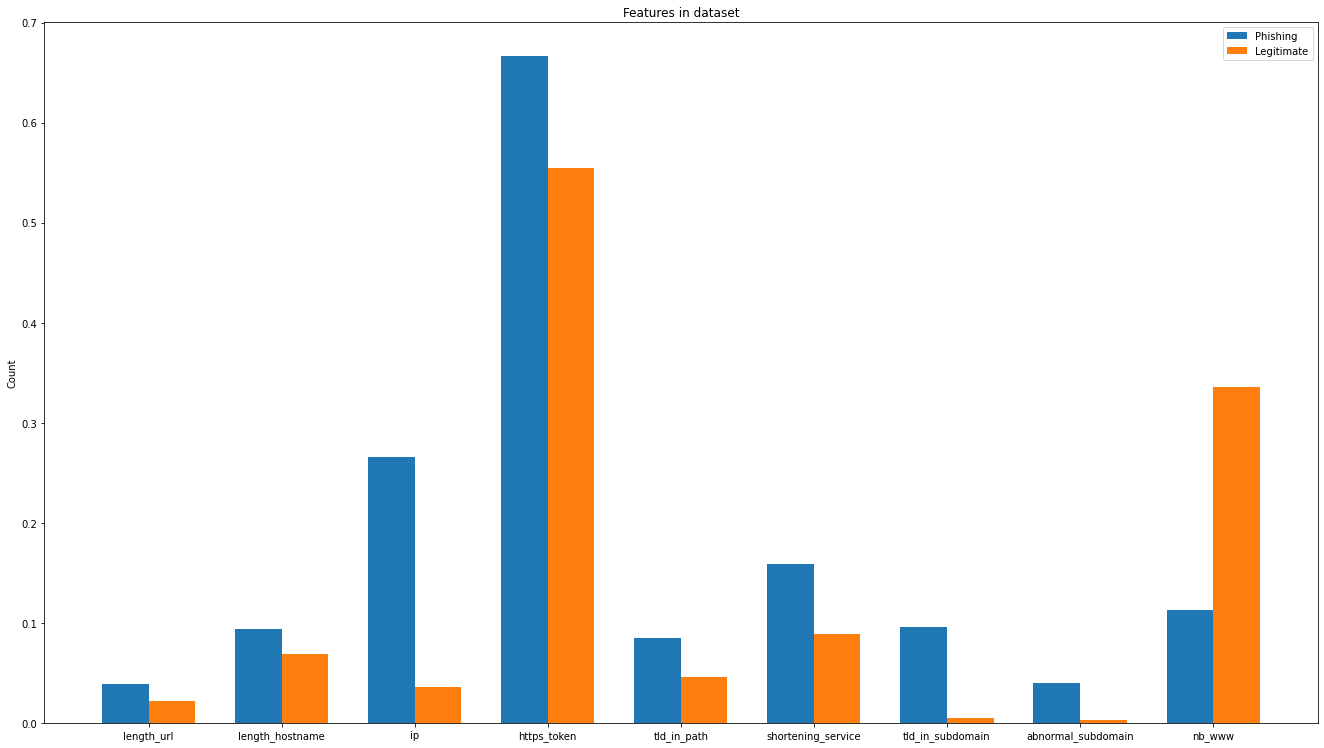
\includegraphics[width=\linewidth]{bar_1.png}
 
 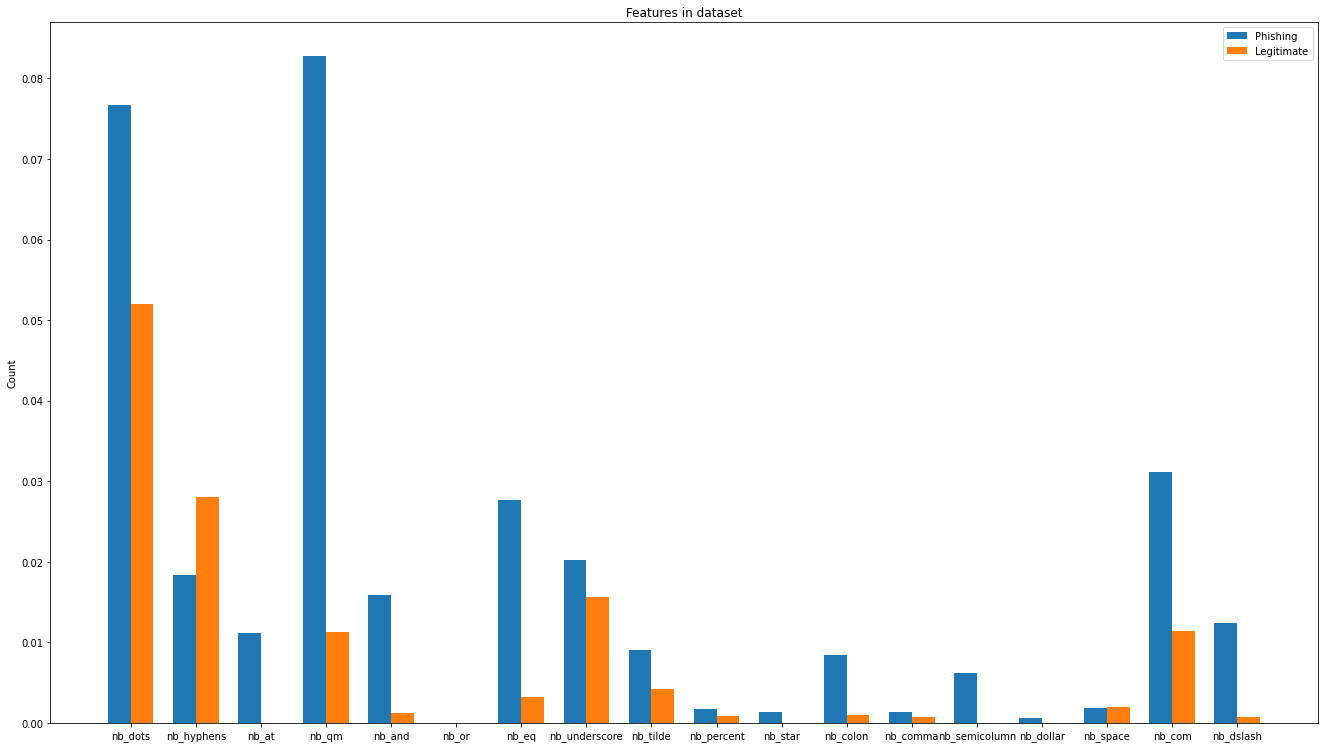
\includegraphics[width=\linewidth]{bar_2.png}
 \captionof{figure}{Double bar graphs depecting how features vary in legitimate and phishing URLs.}
\end{Figure}

\section{Data Interpretation}

Based on \ref{fig:scatter1}, it could be observed that lengthier URLs and hostnames are more probabilistic  to be phishing URLs. 

\\Based on Fig. III and IV, the following observations could be made:

\begin{enumerate}

\item The length of domain names and URLs are longer for phishing URLs.
\item Majority of URLs having an IP address instead of a domain name, were identified to be phishing. 
\item Phishing websites were found to be  using URL shorteners, and did not have SSL support.
\item Most legitimate websites had $www$ in their URL.
\item The number  of phishing websites that had a top-level domain name as a subdomain or as a path was comparatively high.
\item The number of occurrences of special characters such as dots, at, question marks, ampersands, underscores, tildes, stars, colons, commas, etc were found to be more in phishing URLs rather than legitimate URLs . However, the count of hyphens were found to be more in legitimate URLs.

\end{enumerate}

\section{Python packages used}

The following python packages were used in order to build, train, and compare various machine learning models. 

\begin{itemize}
\item scikit-learn - It is a machine learning library that provides various classification, regression and clustering algorithms, and related tools to test, train, and validate the generated model. This library was used in the initial stage  of the project, in order to find a best suitable algorithm.
\item Matplotlib - It is a data visualization library in Python which is used to plot graphs. The library was used in this project to analyze results graphically. 
\item Pandas - It is a software library written for the Python programming language for data manipulation and analysis
\item NumPy - It is a Python library used for working with arrays. It also has functions for working in domain of linear algebra, fourier transform, and matrices.

\end{itemize}

\section{Model Selection}

In this section, we choose four different supervised machine learning algorithms, and analyze their performance separately on the dataset. The best algorithm would be selected for implementation. \\

The algorithms chosen are as follows:

\begin{enumerate}
\item K-Nearest Neighbor Algorithm (KNN)
\item Support Vector Machine (SVM)
\item Gaussian Naive Bayes Classifier
\item Decision Tree Algorithm
\end{enumerate}

The results has been summarized in the following section. 

\subsection{Analysis}

The code used to build and compare the models discussed in this section has been uploaded in the project folder.

\subsubsection{K-Nearest Neighbor Algorithm (KNN)}

The k-nearest neighbors (KNN) algorithm is a supervised machine learning algorithm that can be used to solve both classification and regression problems. 

\\The algorithm was run on the dataset with varying values of k, and the best average accuracy gained was 0.83, with K-Fold Cross Validation, with the number of nearest neighbours as 3. \\

\begin{Figure}
  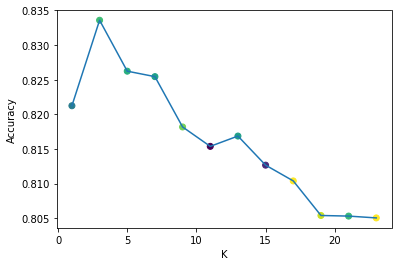
\includegraphics[width=\linewidth]{images/knn-accuracy.png}
  \captionof{figure}{Plot showing accuracy of KNN Algorithm with varying values of K}
  \label{fig:knnvaryingk}
\end{Figure}

\subsubsection{Support Vector Machine (SVM)}

Support vector machines (SVMs) are a set of supervised learning methods used for classification and regression problems. The Support Vector Machine algorithm gave an average accuracy of 0.77 with RBF Kernel. A lowest score of 0.65 was obtained with Sigmoid Kernel. \\

\begin{Figure}
  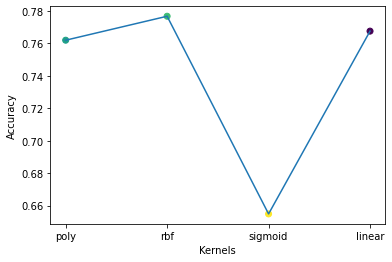
\includegraphics[width=\linewidth]{svm_accuracy}
  \captionof{figure}{Plot showing accuracy of SVM Algorithm with various kernels.}
  \label{fig:svmkernels}
\end{Figure}

\subsubsection{Gaussian Naive Bayes Classifier}

Gaussian Naive Bayes is a variant of Naive Bayes that follows Gaussian normal distribution and supports continuous data. \\

Gaussian Naive Bayes classifier yielded an average accuracy of 0.61. 

\subsubsection{Decision Tree Algorithm}

Decision Tree is a Supervised learning technique that can be used for both classification and Regression problem. It is a tree-structured classifier, where internal nodes represent the features of a dataset, branches represent the decision rules and each leaf node represents the outcome. \\

Decision Tree Algorithm yielded an average accuracy of 0.82. 

\subsection{Summary}

The results obtained from each algorithm has been summarized in the table below.

\begin{center}
\begin{minipage}[t]{.45\textwidth}
\begin{tabular}{@{}lllll@{}}
\toprule
\textbf{Algorithm}                  & Accuracy Obtained &  &  &  \\ \midrule
\textbf{KNN}                  & 0.83 &  &  &  \\ 
\textbf{SVM}                  & 0.77 &  &  &  \\
\textbf{Gaussian Naive Bayes} & 0.61 &  &  &  \\
\textbf{Decision Tree}                & 0.82 &  &  &  \\ \bottomrule
\end{tabular}
\end{minipage}
\end{center}

\begin{Figure*}
  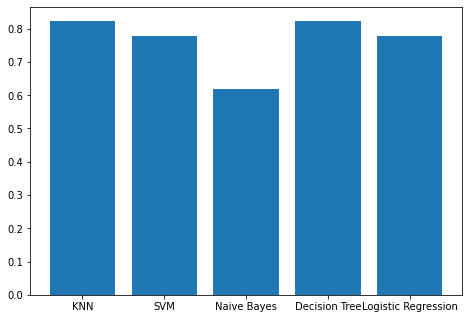
\includegraphics[width=\linewidth]{accuracy_comparison.png}
  \captionof{figure}{Comparison of various machine learning algorithms on the same dataset.}
  \label{fig:algocomparison}
\end{Figure*}


From the observations stated above, the KNN Algorithm appears as a best choice for this problem. We implemented KNN Algorithm, and the implementation has been discussed in the next section.



\section{Implementing KNN}

The following are the requirements to implement the KNN Algorithm. 

\begin{enumerate}
\item Shuffle the dataset in order to reduce the problem of overfitting.
\item Split dataset into test, train and validation datasets.
\item A function to calculate Euclidean Distance.
\item A method to find K nearest neighbours of a given datapoint.
\item A classifier function that classifies a datapoint into phishing or legitimate, on the basis of nearest neighbours.
\item A method to measure accuracy of the implemented algorithm.
\end{enumerate}

The required methods were implemented and has been documented in ipynb files uploaded in the project folder.
\end{multicols}

\subsection{Source Code}

\subsubsection{Loading dataset}

\begin{lstlisting}
# Load the cleaned dataset from Phase - 1

data = pd.read_csv('final_dataset.csv')

# Shuffle the dataset usnig Numpy Random Permutation
shuffle_index = np.random.permutation(data.shape[0])
data = data.iloc[shuffle_index]


# Use 70% of the dataset for training, and remaining 30% for testing.
# In[4]:
train_size = int(data.shape[0]*0.7)

# In[5]:
train_df = data.iloc[:train_size,:] 
test_df = data.iloc[train_size:,:]

train = train_df.values
test = test_df.values

y_true = test[:,-1]

\end{lstlisting}

\pagebreak

\subsubsection{Euclidean Distance}

The euclidean distance betweet two vectors is calculated using the formula : \\ 

 d\left( p,q\right)   = \sqrt {\sum _{i=1}^{n}  \left( q_{i}-p_{i}\right)^2 } 

\\ The same is implemented in Python below.

\begin{lstlisting}
from math import sqrt

def euclidean_distance(x_test, x_train):
    """
    Calculates Euclidean distance between two given vectors.
    Args: Vector A, Vector B
    Returns: Distance between two given vectors.
    """
    
    distance = 0
    
    for i in range(len(x_test)-1):
        distance = distance + (x_test[i] - x_train[i])**2

    return sqrt(distance)
\end{lstlisting}

\subsubsection{Finding N nearest neighbors}

\begin{lstlisting}
def find_n_neighbors(x_test, x_train, N):
    """
    Function that finds N nearest neighbors of a vector by calculating euclidean distance between them.
    
    Args: 
        x_test : Vector A, 
        x_train : Set of vectors
        N : Number of nearest neighbors required
        
    Returns:
        N Closest vectors to vector A
        
    """
    
    distances = []
    data = []
    
    # For each datapoint in training set,
    # find the distance from X_test vector
    for row in x_train:
        distances.append(euclidean_distance(x_test, row))
  
    # Sort distances and return N records
    distances = np.array(distances)
    data = np.array(x_train)
    sort_indexes = distances.argsort()             
    data = data[sort_indexes]  
    
    return data[:N]               
\end{lstlisting}

\pagebreak

\subsubsection{The KNN Function}

\begin{lstlisting}
def knn(x_test, x_train, N):
    """
        The KNN Classifier Function
        Arguments:
            x_test : Test point
            x_train : Set of N vectors
            N : no of nearest neighbours
        Returns:
            Class of test point   
    """
    
    positive = 0
    negative = 0

    # Find N nearest neighbours
    # Class of the test point will be
    # class of majority of nearing classes
    neighbors = find_n_neighbors(x_test, x_train, N)
    
    for i in neighbors:
        
        if i[-1] == 0:
            negative += 1
        else:
            positive += 1
        
    if negative > positive:
        return 0
    
    return 1
\end{lstlisting}

\subsection{Calculating Accuracy}

\begin{lstlisting}
def calculate_accuracy(y_true, y_pred):
    """
    Function to calculate accuracy given predicted classes, and originally correct classes.
    Args:
        y_true : Actual true classes
        y_pred : Classes predicted using KNN 
        
    Returns:
        Accuracy 
    """
    correct = 0
    
    for i in range(len(y_true)):
        if y_true[i] == y_pred[i]:
            correct += 1
            
    accuracy = correct / len(y_true)
    return accuracy
\end{lstlisting}

\begin{multicols}{2}

\subsection{Result}

\begin{Figure}
  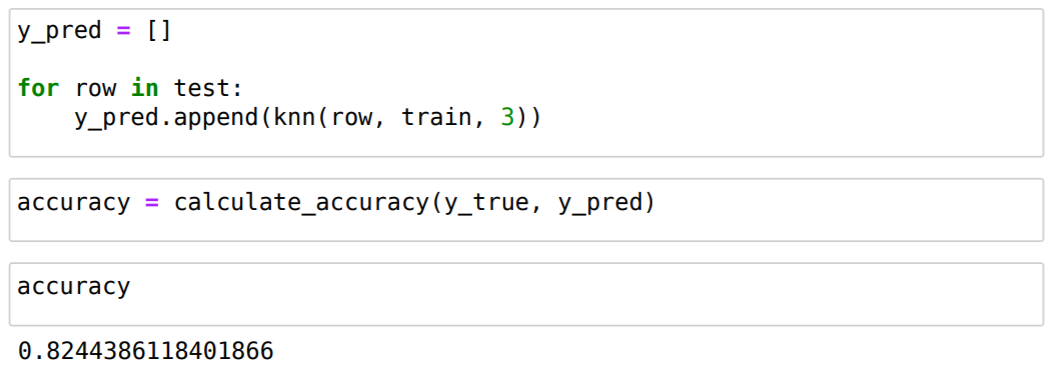
\includegraphics[width=\linewidth]{impl6.png}
\end{Figure}

Upon running the KNN function with k = 3, an accuracy of 0.82 was obtained on unseen data. 

\section{Conclusion}

A machine learning algorithm (K nearest neighbors classifier) was developed from scratch in order to classify phishing and legitimate URLs. 

\href{https://amritauniv-my.sharepoint.com/:f:/g/personal/yadhukrishna_am_students_amrita_edu/ErRa1KKzBQROssk2Y6KyZmoBZmovAkmMdeOQCI79fXT4pQ}{Link to project folder} 

\end{multicols}

\end{document}

@MISC{Anu:2013,
author = {Aggarwal, Anupama},
title = {This is how you cite a website in latex},
month = may,
year = {2013},
howpublished={\url{http://precog.iiitd.edu.in/people/anupama}}
}

\setstretch{1}  %reduce bibliography line spacing
\printbibliography

\end{document}
